\documentclass{sig-alternate}

\usepackage{times}

\usepackage{url}
\urlstyle{it}
\usepackage{graphicx}
\usepackage{graphics}
\usepackage{subfig}
\usepackage{longtable}
\usepackage{array}
\usepackage{multirow}
\usepackage{textcomp}
\usepackage{framed,color}
% Paragraphs
\newcommand{\spara}[1]{\smallskip\noindent{\bf #1}}
\newcommand{\mpara}[1]{\medskip\noindent{\bf #1}}
\newcommand{\para}[1]{\noindent{\bf #1}}

\clubpenalty=10000
\widowpenalty=10000

%% Define a new 'leo' style for the package that will use a smaller font.
\makeatletter
\def\url@leostyle{%
  
\@ifundefined{selectfont}{\def\UrlFont{\sf}}{\def\UrlFont{\scriptsize\ttfamily}}}
\makeatother
%% Now actually use the newly defined style.
\urlstyle{leo}




\begin{document}
%\conferenceinfo{WISDOM'13,}{August 11 2013, Chicago, IL, USA}
 

%\crdata{978-1-4503-2332-1/13/08}
%\CopyrightYear{2013}

% Place holder, can be changed if wanted
\title{ A time-series classification model for Twitter opinion lexicon expansion}

% Propose this new titlte
% Supervised opinion lexicon expansion from automatically labelled tweets

\numberofauthors{3}
\author{
% You can go ahead and credit any number of authors here,
% e.g. one 'row of three' or two rows (consisting of one row of three
% and a second row of one, two or three).
%
% The command \alignauthor (no curly braces needed) should
% precede each author name, affiliation/snail-mail address and
% e-mail address. Additionally, tag each line of
% affiliation/address with \affaddr, and tag the
% e-mail address with \email.
%
% 1st. author
\alignauthor
Felipe Bravo-Marquez\\
	\affaddr{Department of Computer Science, University of Waikato, New Zealand}\\
	\email{fjb11@students.waikato.ac.nz}
\alignauthor Eibe Frank\\
       \affaddr{Department of Computer Science, University of Waikato, New Zealand}\\
       \email{eibe@waikato.ac.nz}
\alignauthor Bernhard Pfahringer\\
       \affaddr{Department of Computer Science, University of Waikato, New Zealand}\\
       \email{bernhard@waikato.ac.nz}
}



\maketitle

\begin{abstract}
Opinion lexicons, which are lists of terms labelled by sentiment, are widely used resources to support automatic sentiment analysis of textual passages. However, these resources exhibit important limitations when applied to social media messages such as tweets (posts in Twitter), because they are unable to capture the diversity of informal expressions commonly found in this type of media. In this article, we propose a process to automatically categorise Twitter words into three sentiment classes: positive, neutral, and negative. The expansion is done through a supervised learning process in which word-level attributes are calculated from a multi-dimensional time-series, and a seed lexicon of labelled words is used as the training dataset. The time-series are extracted from a temporal collection of automatically labelled tweets representing the relationship between the word and the sentiment expressed in the tweets where it occurs. Our experimental results show that our method outperforms the word-level sentiment classification performance obtained by semantic orientation, a well known state-of-the-art measure for establishing world-level sentiment. Additionally, we show that our expanded lexicon produces significant improvements when used for message-level polarity classification of tweets.


\end{abstract}

\category{I.2.7.7}{Artificial Intelligence}{Natural Language Processing}[Text Analysis]

\terms{Experimentation, Measurement}

\keywords{Lexicon Expansion, Sentiment Analysis, Twitter}


\section{Introduction}\label{sec:intro}

Several sentiment analysis methods rely on lexical resources for evaluating the sentiment of a text passage, in particular they often rely on an opinion lexicon. An opinion or sentiment lexicon is a dictionary of opinion words with their corresponding sentiment values. Lexicons can be used to compute the polarity of a message by aggregating the orientation values of the opinion words found in the document \cite{Wiebe2000}. They have also proven to be useful when used to extract features in supervised classification schemes~\cite{jiang2011target, kouloumpis2011twitter,Zirn20011}. 

Social media platforms and, in particular, microblogging services such as \textbf{Twitter}\footnote{\url{http://www.twitter.com}}, are increasingly being adopted by people to access and publish information about a great variety of topics. Sentiment analysis applied to social media posts has received an increasing interest due to its importance in a wide range of fields such as business, sports, and politics. However, the language used in Twitter provides substantial challenges for sentiment analysis. The words used in this platform include many abbreviations, acronyms, and misspelled words which are not observed in traditional media and are not covered by most popular lexicons such as OpinionFinder \cite{Wilson2005}, SentiWordnet \cite{esuli2006}, and the Harvard General Inquirer \cite{stone66}. The diversity and sparseness of these informal words make the manually creation of a Twitter-oriented opinion lexicon a time-consuming task.

% Words can be positive, negative, or neutral depending on the context

In this article we propose a supervised framework for opinion lexicon expansion for the language used in Twitter.  Taking SentiWordnet as inspiration, each word in our expanded lexicon has a probability distribution, describing how positive, negative, and neutral it is.  Additionally, all the entries of the lexicon are associated with a corresponding part-of-speech tag. We believe that estimating the sentiment distribution of POS-tagged words according the three opinion-related properties may be useful for developing Twitter-specific sentiment applications due to the following reasons:

\begin{enumerate}
%\item There are some words in which its opinion-related properties can change from one domain to another, e.g., the word \emph{small} is positive when referring to a queue in a bank but negative when referring to a hotel room. These type of words could be represented by having probabilities greater than zero for both positive and negative classes.
\item A word can present certain levels of intensity \cite{ThelwallBP12} for a specific sentiment category e.g., the word \emph{awesome} is more positive than the word \emph{adequate}. The estimated probabilities could be used to represent these levels of intensities.

\item  The neutral score provided by the lexicon could be useful for discarding non-opinion words in text-level polarity classification tasks. This can be easily done  taking the class with the maximum probability and discarding words classified as neutral. On the other hand, unsupervised lexicon expansion techniques such as semantic orientation \cite{Turney2002} provide a single numerical score for each word. It is no clear how to find a threshold for using this score in neutrality detection. 

\item   Homographs, which are  words that share the same spelling but have different meanings, should  have different lexicon entries for each different meaning. By relying on POS-tagged words, homographs with different POS-tags will be disambiguated \cite{wilks1998grammar}. For instance, the word \emph{apple}  will receive different sentiment scores when used to refer to a common noun (a fruit) or a proper noun (a company). 

\end{enumerate}


The proposed methodology takes a collection of tweets labelled according to their polarity to establish a polarity-related time series for each POS-tagged word in the tweets and uses features extracted from this time series in relation with the labels provided by a seed lexicon to train a word-level sentiment classifier. The seed lexicon is taken from the union of different hand-made lexicons after discarding all polarity clashes from the intersection. Furthermore, the tweets from the collection are labelled using a semi-supervised heuristics to avoid the expensive costs of data annotation: \emph{emoticon-based annotation}. In this approach, only tweets having positive or negative emoticons are considered and labelled according to the polarity indicated by the emoticon \cite{go2010}. 

%In the second approach, the tweets are classified into classes positive, negative and neutral using two sentiment analysis tools: \emph{SentiStrength}\footnote{\url{http://sentistrength.wlv.ac.uk/}} and \emph{Sentiment140}\footnote{\url{http://www.sentiment140.com/}}. Afterwards, all tweets in which both methods disagree are discarded. 


Our word-level time series are computed from two different criteria: Semantic Orientation (SO) \cite{Turney2002}, which is based on the mutual information between word and sentiment class, and Stochastic Gradient Descent (SGD) score, which learns a linear relationship between word and sentiment class.

The proposed procedure can be summarised in the following steps:

\begin{enumerate}
\item Collect tweets from the domain and the time period for which the lexicon needs to be expanded. 
\item Label the collection with sentiment classes in an automatic way.
\item Tag all the words using a part-of-speech tagger.
\item Calculate word-level time-series for all tagged words and extract sentiment features from them.
\item Label the sentiment of the words that match an existing hand-made polarity lexicon.
\item Train a word-level classifier using the word-level features and the words labels from the seed lexicon.
\item Use the trained classifier to estimate the polarity distribution of the remaining unlabelled words.
\end{enumerate}
 
%Briefly explain the experiments 
As will be discussed in Section~\ref{sec:related}, the automatic expansion of Twitter  opinion words has been studied before \cite{Mohammad2013, avaya2013, Zhou2014}. In all these works, the expansion was conducted using semantic orientation, which is an unsupervised measure.  
To the best of our knowledge, this is the first article in which the lexicon expansion of Twitter opinion words is studied and evaluated using POS disambiguation and supervised learning. Additionally, this is the first study in which scores for positive, negative, and neutral opinion-related properties are provided for Twitter-specific expressions.


%It is important to remark that a supervised word labelling approach based on a seed lexicon provides flexibility in determining the desired nature of the polarity label of the expanded words. For instance, we can compute a categorical label through classification or a numerical score through regression. On the other hand, when the lexicon is created from  unsupervised measures such as semantic orientation is it not clear how to transform these values into the desired labels.  


%This is the first study comparing two different mechanisms for automatic labelling tweets for lexicon expansion (Emoticon Labels and Consensus of methods).

%This is the first study combining the semantic orientation measure with POS tags (POS tags were used before as filters to discard words from POS that are unlikely to express an opinion). This is the first study in Twitter lexicon expansion including the detection of neutral words. This is the first study in which semantic orientation is compared and combined with SGD scores. 
 
We test our approach on two collections of automated labelled tweets. Our results indicate that our supervised framework outperforms the classification accuracy obtained by  semantic orientation when the detection of neutral words is included. We also evaluate the usefulness of the expanded lexicon for message-level polarity classification of tweets, showing significant improvements in performance.   
 
This article in organised as follows. In Section~\ref{sec:related} we provide a review of existing work in opinion lexicon expansion. In Section~\ref{sec:tweetlab} we describe the seed lexicon used to label the words for the training set. In Section~\ref{sec:seed_lex} we explain the mechanisms studied to automatically create collections of labelled tweets.
 The creation of our word-level time-series is described in Section~\ref{sec:feat}, together with the features used for training the classifier. In Section~\ref{sec:lex_expand} we present the experiments we conducted to evaluate the proposed approach and we also discuss the obtained results. The main findings and conclusions are discussed in Section~\ref{sec:conc}.

\section{Related Work}\label{sec:related}
There are basically two type of resources which can be exploited for lexicon expansion: a  thesaurus and a corpus of documents. The simplest approach using a thesaurus such as WordNet\footnote{\url{http://wordnet.princeton.edu/}} is to expand a seed lexicon of labelled opinion words using synonyms and antonyms from the lexical relations provided by the thesaurus 
\cite{Liu2004,Kim2004}. The hypothesis behind this approach is that synonyms may have the same polarity and antonyms may have the opposite. This process is normally iterated several times.
In \cite{kamps2004} a graph was created using WordNet adjectives as vertices and the synonym relation as edges. The orientation of a term is determined by its relative distance from two seed terms \emph{good} and \emph{bad}. In \cite{Esuli2005} a supervised classifier was trained using a seed of labelled words which was obtained through synonyms and antonyms expansion. For each word, a vector space model is created from the definition or \emph{gloss} provided by the WordNet dictionary. This representation is used to train a word-level classifier that is used for lexicon expansion. An equivalent approach was applied later to create SentiWordnet\footnote{\url{http://sentiwordnet.isti.cnr.it/}} in \cite{esuli2006, Baccianella2010}. In SentiWordNet each WordNet \emph{synset} or group of synonyms is  annotated into classes positive, negative and neutral in the range $[0,1]$.    

A limitation of thesaurus-based approaches is their inability to capture domain dependent words. On the other hand, corpus-based approaches exploit syntactic or co-occurrence patterns to expand the lexicon to the words found within a collection of documents. 
In \cite{Hatziva1997}, the proposed method starts with a set of adjectives whose polarity is known and then discovers the polarities of new adjectives using some linguistic patterns from a corpus of documents. The authors show, using log-linear regression, that conjunctions between adjectives provide indirect information about the orientation. For example, adjectives connected with the conjunction ``and'' tend to have the same orientation and adjectives connected with the conjunction ``but'' tend to have opposite orientation. This approach allows the extraction of domain-dependent information and the adaptation to new domains when the corpus of documents is changed. 

In \cite{Turney2002, turney2003measuring}, the expansion is done through a measure referred to as \emph{semantic orientation} which is based on the the point-wise mutual information (PMI) between two random variables:
\begin{equation}
 \operatorname{PMI}(term_{1}, term_{2})= \log_{2} \left ( \frac{Pr(term_{1} \wedge term_{2})}{Pr(term_{1})Pr(term_{2})} \right )
\end{equation}

The semantic orientation of a word is the difference between the PMI of the word with a positive emotion and a negative emotion. Different ways have been proposed to represent the joint probabilities of words and emotions. In Turney's work \cite{Turney2002, turney2003measuring} they are estimated using the number of hits returned by a search engine in response to a query composed of the target word together with the word ``excellent'' and another query using the word ``poor'' in the same way.  

The same idea was used for Twitter lexicon expansion in \cite{Mohammad2013, avaya2013, Zhou2014}. All these works model the joint probabilities from collections of tweets labelled in automatic ways. In \cite{avaya2013} the tweets are labelled from a trained classifier using thresholds for the different classes to ensure high precision. In \cite{Zhou2014}, the tweets are labelled from emoticons to create domain-specific lexicons. In \cite{Mohammad2013}, tweets are labelled from emoticons and hashtags associated with emotions to create two different lexicons. These lexicons were tested for tweet-level polarity classification. 




\section{Ground-Truth word polarities}\label{sec:seed_lex}
In this section, we describe the seed lexicon used to label the training dataset for our word sentiment classifier. There are two main properties that vary from one lexicon to another: the way in which the lexicon is built and the nature of the sentiment label. Lexicons can be created manually or automatically. Manually created lexicons tend to be smaller and less noisy than automatically made lexicons \cite{BravoMarquez2014}. 

 The labels can be categorical, with classes -positive, negative, and neutral- (in some cases neutral words are not considered), or numerical, representing the strength of the polarity (e.g., from -5 to 5). The labels can also express additional emotional states.


As we need to reduce the noise in our training data, we consider the following hand-made lexicons for data labelling:
\begin{itemize}
\item \emph{MPQA Subjectivity Lexicon}:  This lexicon was created by Wilson et al.~\cite{Wilson2005} and is part of OpinionFinder\footnote{\url{http://mpqa.cs.pitt.edu/opinionfinder/opinionfinder_2/}}, a system that automatically detects subjective sentences in document corpora. The lexicon has positive, negative, and neutral words. 
\item \emph{Bing Liu}: This lexicon is maintained and distributed by Bing
Liu\footnote{\url{http://www.cs.uic.edu/~liub/FBS/sentiment-analysis.html}} and
was used in several papers authored or co-authored by him~\cite{LiuBook}. The lexicon has positive and negative entries. 
\item \emph{Afinn}:  This strength-oriented lexicon \cite{Finn2011} has positive words scored from 1 to 5 and negative words scored from -1 to -5. It include slang and obscene words and also acronyms and Web jargon. We tagged words with negative and positive scores to   negative and positive classes respectively.
\item \emph{NRC emotion Lexicon}: This emotion-oriented lexicon was created by Mohammad and Turney~\cite{Saaif2012}  by conducting a tagging process in the crowdsourcing Amazon Mechanical Turk platform. In this lexicon, the words are annotated according to eight emotions: joy, trust, sadness, anger, surprise, fear, anticipation, and disgust, and two polarity classes: positive and negative. There are many words that are not associated with any emotional state which were tagged as neutral. In this work, we consider positive, negative, and neutral tags from this lexicon. 
\end{itemize}

We create a meta-lexicon by taking the union of these resources and discarding all words where a polarity clash is observed. A polarity clash is a word that receives two or more different tags in the union of lexicons. Our meta-lexicon is a hand-made lexical resource including positive, negative, and neutral words with mutually exclusive classes. The number of words for the different polarity classes in the different lexicons is displayed in Table~\ref{tab:lexstats}.   


\begin{table}[htbp]
\begin{center}
\begin{tabular}{l|c|c|c}
\hline
 & Positive & Negative & Neutral \\ \hline
AFINN & 564 & 964 & 0 \\ 
Bing Liu & 2003 & 4782 & 0 \\ 
MPQA & 2295 & 4148 & 424 \\ 
NRC-Emo & 2312 & 3324 & 7714 \\ \hline
Union & 4331 & 7004 & 8013 \\ 
Meta-Lex & 3730 & 6368 & 7088 \\ \hline
\end{tabular}
\end{center}
\caption{Lexicon Statistics}
\label{tab:lexstats}
\end{table}

From the table we can observe that the number of words per class is significantly reduced after removing the clashes from the union. The total number of clashes is 1074 and a sample of them in presented in Figure~\ref{fig:word_clash}. 
\begin{figure}[ht]
	\centering
	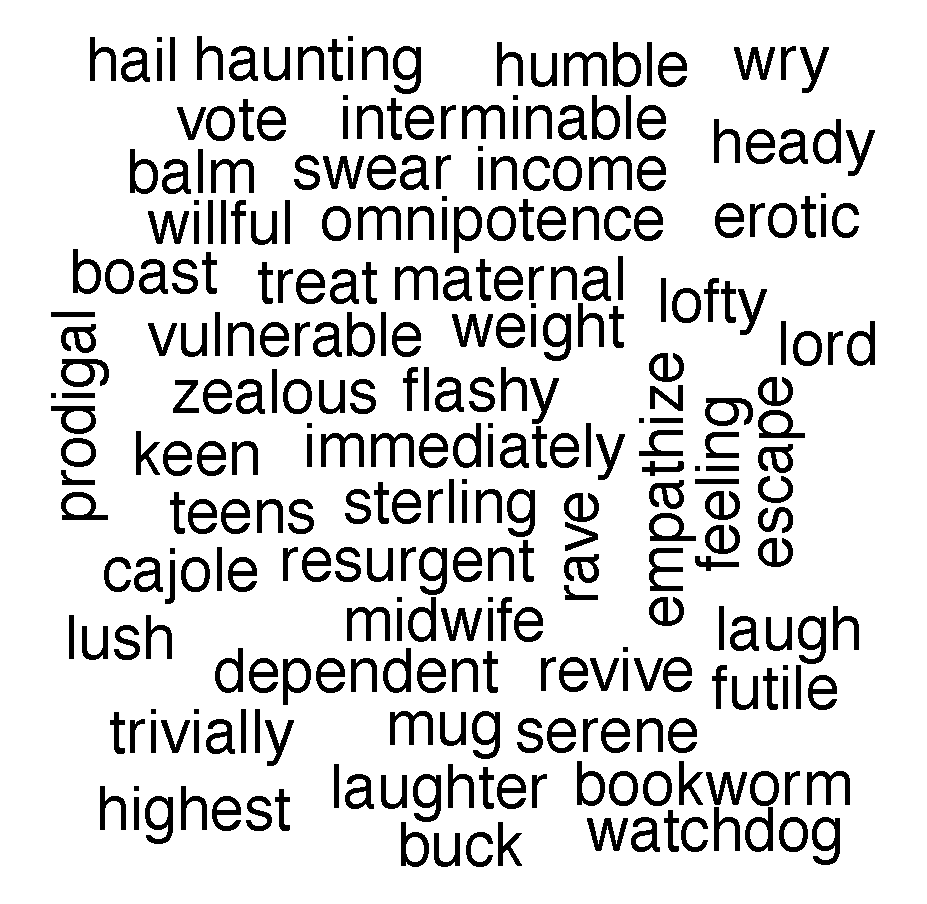
\includegraphics[scale=0.3]{clashes.pdf}
	\caption{Polarity clashes}
	\label{fig:word_clash}
\end{figure}


This high number of clashes found among different hand-made lexicons indicates two things: 1) Different human annotators can disagree when tagging a word to polarity classes. 2) There are several words that can belong to more than one sentiment class.  
Due to this, we can say that word-level polarity classification is a hard and subjective problem.  



% POS tags are not provided

\section{Obtaining labelled tweets}\label{sec:tweetlab}

In order to calculate our word-level time-series we require a collection of time-stamped tweets with their corresponding polarity labels. 

We study two different ways for automatically labelling a collection of tweets. 
The first one is the emoticon-based annotation approach in which tweets exhibiting positive :) and negative :( emoticons are labelled according to the emoticon's polarity. Afterwards, the emoticon used to label the passage is removed from the content. A limitation of this approach is its inability to capture neutral tweets. 

The second approach applies a consensus of existing tweet classification methods. It considers tweets labelled to classes positive, negative, and neutral using two different methods: Sentiment140 and SentiStrength. All tweets where the two methods disagree are discarded.  

Sentiment140\footnote{\url{http://www.sentiment140.com/}} is a Web application that classifies tweets using a maximum entropy classifier \cite{go2010} trained from a corpus of tweets labelled with the emoticon-based annotation approach. SentiStrength is a lexicon-based sentiment evaluator focused on social media messages written in English \cite{ThelwallBP12}. SentiStrength relies on a polarity lexicon, a negating word list, and an emoticon list, among other attributes, to analyse the content. The method returns a positive score, a negative score, and a polarity class with values positive, negative, and neutral.

Several researchers claim that general purpose lexical resources cannot reflect domain-specific language usage \cite{Choi2009, Zhou2014}. This means that the word polarities of the expanded lexicon will reflect the domains found in the collection from which the lexicon is built.  In this work, with the aim of creating general purpose lexicons, we consider three  collections of tweets covering multiple topics: The Edinburgh corpus (ED) \cite{Petrovic2010}, the Stanford Sentiment corpus (STS) \cite{go2010}, and the Consensus collection (CON). All these collections were gathered from  two Twitter APIs: the streaming API\footnote{\url{https://dev.twitter.com/streaming/overview}}, from which a real time sample of public posts can be retrieved, and the search API\footnote{\url{https://dev.twitter.com/rest/public/search}}, which allows the submission of queries composed by key-terms.

The ED corpus has 97 million tweets which were collected using the Twitter streaming API from a period spanning November 11th 2009 until February 1st 2010. This collection includes tweets in multiple languages. As was done in \cite{bifet2010}, non-English tweets were filtered out, and tweets exhibiting positive or negative emoticons were annotated using the emoticon-based approach. The remaining tweets were discarded.

The STS corpus was created by periodically sending queries :) and :( to the Twitter REST API between April 6th 2009 to June 25th 2009. All the tweets in this collection are written in English. The collection was labelled using the emotion-based annotation approach.

The CON corpus was gathered by periocally sending queries to the Twitter REST API from 12th April to 22nd July 2012 regarding multiple topics. A parameter was specified to retrieve tweets written only in English. The topics were chosen from different domains that are frequently discussed in Twitter: politicians, countries, companies and long-standing topics. For the case of politicians, the studied period coincided with the electoral campaign of the U.S. 2012 presidential elections. We retrieved tweets related to both Republican and Democrat candidates Mitt Romney and Barack Obama. Additionally, we
tracked tweets on the U.K prime minister David Cameron and the U.S. Democrat politician Hillary Clinton. We selected countries which face either an internal or external conflict situation: Iran, Israel and North Korea. We also tracked tweets related to two of the most influential high-tech companies in the world: Google and Facebook.  Finally, we selected two long-standing topics that are constantly discussed by the public: abortion and global warning. The total number of tweets in the collection is $5,175,984$. All these tweets were classified using Sentiment140 and SentiStrength and labelled using the consensus of methods. Hence, that all tweets were the two methods assigned a different class were discarded.



\begin{table}[htbp]
\begin{center}
\begin{tabular}{l|c|c|c}
\hline
 & ED & STS & CON \\ \hline
Positive & $1,813,705$ & $800,000$ & $535,192$ \\ 
Negative & $324,917$ & $800,000$ & $295,349$ \\ 
Neutral & 0 & 0 & $1,660,703$ \\ \hline
Total & $2,138,622$ & $1,600,000$ & $2,491,244$ \\ 
\end{tabular}
\end{center}
\caption{Collection statistics}
\label{tab:colstats}
\end{table}


The number of tweets for each polarity class in the three corpora is given in Table~\ref{tab:colstats}. We can observe that when using the streaming API (ED) positive emoticons occur much more frequently than negative ones. We can also see in the CON corpus that neutral tweets occur much more frequently than positive and negative tweets.



\section{Word-level features}\label{sec:feat}

The word-level features proposed in this work exploit the temporal structure of a collection of polarity-labelled tweets. All the tweets from the collection are lowercased, tokenised and POS-tagged. We use the TwitterNLP library \cite{twitterNLP} that provides a  tokeniser and a tagger specific for the language used in Twitter. The tagger includes  nominal words classes, open and closed word classes, and Twitter specific classes such as hashtags, user mentions and emoticons. We prepend a POS-tag prefix to each word in order to differentiate homographs exhibiting different POS-tags.

We  treat the time-sorted collection of tweets as a data stream and create two types of time-series for each POS-tagged word observed in the vocabulary: the SGD series, and the SO series.

The first time-series is calculated by incrementally training a linear support vector machine using a stochastic gradient descent (SGD) online learning process. The weights of this linear model correspond to POS-tagged words that are updated in an incremental fashion. We  optimise the hinge loss function with an $L_2$ penalty and a learning rate equal to $0.1$:
 
\begin{equation}
\frac{\lambda}{2}||w||^2+\sum [1- (y \mathbf{xw} +b) ]_{+}.
\end{equation}

The variables $\mathbf{w}$, $b$, and $\lambda$ correspond to the weight vector, the bias, and the regularisation parameter, respectively. The class labels $y$ are assumed to be in $\{+1,-1\}$, corresponding to positively and negatively labelled tweets, respectively. The regularisation parameter was set to $0.0001$.  As was suggested in \cite{bifet2010}, the model's weights determine how strongly the absence or presence of a word influences the prediction of negative and positive classes.  The SGD time-series is created by applying this learning process to a collection of labelled tweets and storing the word's coefficients in different time windows. We use time windows of $1,000$ examples.  

The second time-series corresponds to the accumulated semantic orientation (SO) introduced in Section~\ref{sec:related}. Let \emph{count} be a function that counts the number of times that a word or a sentiment label has been observed during a certain period of time. We calculate the SO score for each POS-tagged word using the following expression:   

\begin{equation}
 \operatorname{SO}(word) = log_2 \left( \frac{\operatorname{count}(\text{word $\wedge$ pos}) \times \operatorname{count}(\text{neg})}{\operatorname{count}(\text{word $\wedge$ neg}) \times \operatorname{count}(\text{pos})}\right)
\end{equation}


We use time windows of $1,000$ examples and the Laplace correction to avoid the zero-frequency problem. 


\begin{table}[htbp]
\footnotesize
\begin{center}
\begin{tabular}{l|l}
\hline
Feature & Description \\ \hline
mean &  the mean of the time series. \\ 
trimm.mean &  The trimmed mean of the time series. \\ 
median &  The median of the time series \\ 
last.element &  The last observation of the time series.\\ 
sd &  The standard deviation of the time series . \\ 
iqr &  The inter-quartile range. \\ 
sg &  The fraction of times the time series changes its sign. \\ 
sg.diff &  The sg value for the  differenced time series. \\ \hline
\end{tabular}
\end{center}
\caption{Time-series features}
\label{tab:feat}
\end{table}

We create SGD and SO time-series for positive and negative labelled tweets in our three datasets: ED, STS, and CON. We refer to these time-series as \textbf{sgd.posneg} and \textbf{so.posneg}. Additionally, for the CON dataset we calculate two more time-series using neutral and non-neutral tweets. Non-neutral tweets are obtained by combining positive and negative tweets.  We call these time-series \textbf{sgd.neu} and \textbf{so.neu}. 


We rely on our time-series to extract features which are used to train our world-level polarity classifier. These features intend to summarise the main properties of the time-series and are listed in Table~\ref{tab:feat}. It is important to remark that the attribute last.element of the so.posneg time-series would be equivalent to the traditional SO measure. In addition to these time-series features, we include the POS-tag of the word as a nominal attribute.



\section{Lexicon Expansion}\label{sec:lex_expand}


In this section we present our experimental results for word-level polarity classification. We calculated the time-series described in Section~\ref{sec:feat} for the most frequent $10,000$ POS-tagged words found in each of our three datasets. 

\begin{figure}[ht]
\begin{center}
\begin{tabular}{c}
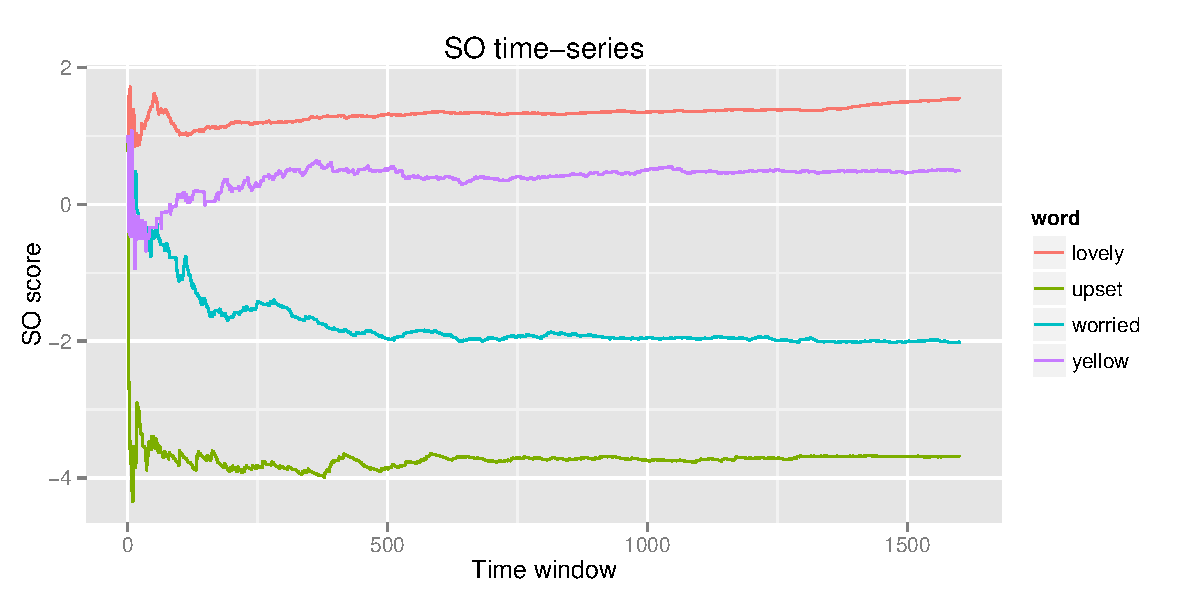
\includegraphics[scale=0.45]{SOseries.pdf} \\
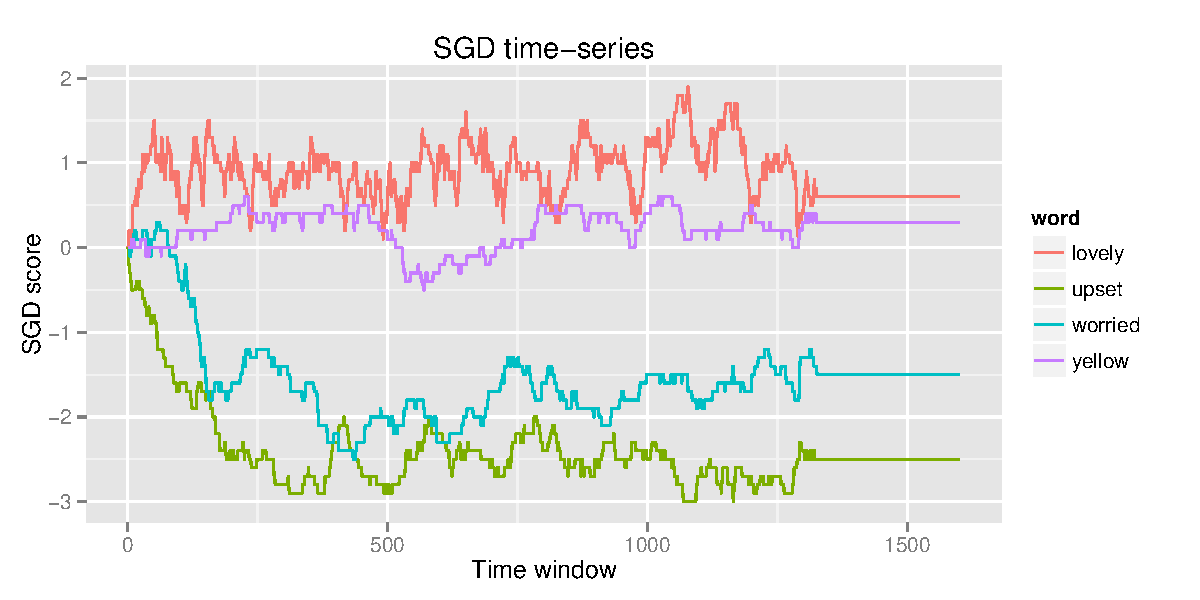
\includegraphics[scale=0.45]{SGDseries.pdf}\\
\end{tabular}
\caption{Word-level time-series}
\label{fig:timeseries}
\end{center}
\end{figure}

The resulting time-series \textbf{sgd.posneg} and \textbf{so.posneg} for a sample of words in the STS dataset is shown in Figure~\ref{fig:timeseries}. We can observe a coherent order in both time-series for positive word \emph{lovely}, neutral word \emph{yellow}, and  negative words \emph{worried}, and \emph{upset}. However, the SO time-series is much more stable than the SGD one. 


The feature values from these words is given in Table~\ref{fig:featex}

\begin{table}[ht]
\footnotesize
\centering
\begin{tabular}{l|llll}
  \hline
Attribute & lovely & yellow & upset & worried \\ 
  \hline
sgd.last &  0.6 &  0.3 & -2.5 & -1.5 \\ 
  sgd.posneg.mean &  0.9 &  0.2 & -2.4 & -1.6 \\ 
  sgd.posneg.trimm.mean &  0.9 &  0.2 & -2.5 & -1.6 \\ 
  sgd.posneg.median &  0.9 &  0.3 & -2.5 & -1.6 \\ 
  sgd.posneg.sd & 0.3 & 0.2 & 0.5 & 0.5 \\ 
  sgd.posneg.sg & 0.0 & 0.0 & 0.0 & 0.0 \\ 
  sgd.posneg.sg.diff & 0.2 & 0.0 & 0.1 & 0.0 \\ 
  sgd.posneg.iqr & 0.5 & 0.3 & 0.3 & 0.3 \\ 
  so.posneg.last &  1.5 &  0.5 & -3.7 & -2.0 \\ 
  so.posneg.mean &  1.3 &  0.4 & -3.7 & -1.8 \\ 
  so.posneg.trimm.mean &  1.3 &  0.4 & -3.7 & -1.9 \\ 
  so.posneg.median &  1.3 &  0.5 & -3.7 & -1.9 \\ 
  so.posneg.sd & 0.1 & 0.2 & 0.2 & 0.4 \\ 
  so.posneg.sg & 0.0 & 0.0 & 0.0& 0.0 \\ 
  so.posneg.sg.diff & 0.5 & 0.4 & 0.4 & 0.4 \\ 
  so.posneg.iqr & 0.1 & 0.1 & 0.1 & 0.1 \\ 
  pos.tag & adjective & adjective & adjective & verb \\ \hline
  label & positive & neutral & negative & negative \\ 
   \hline
\end{tabular}
\caption{Word-level feature example}
\label{fig:featex}
\end{table}



Subsequently, all the words matching the metalexicon were labelled according to the lexicon's polarities. As the lexicon's entries are not POS-tagged, we assumed that all posible POS-tags of a word will have the same polarity. However, we have to be aware that this assumption can introduce noise in the training data. For example, the word \emph{ill} would be labelled as negative for two different POS-tags: adjective, and nominal+verbal contraction. As this word is very likely to express a negative sentiment when used as an adjective, it would be unlikely to express a negative sentiment when used to refer to the  contraction \emph{I'll}. A simple technique to deal with this problem will be discussed later in this section.



A plot of the mean values of SGD and SO scores for the three different categories -positive, negative, and neutral- is shown in Figure~\ref{fig:sosgd}.


\begin{figure}[ht]
	\centering
	%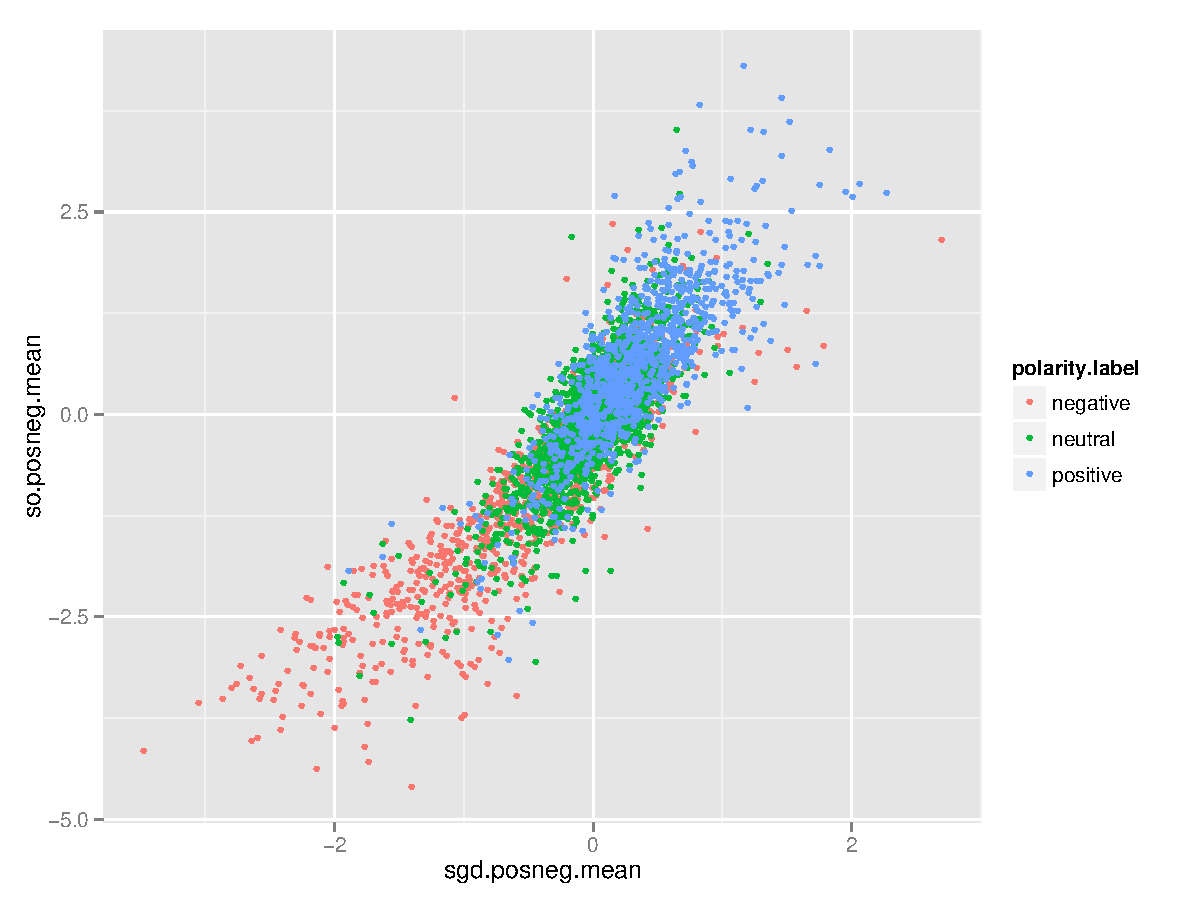
\includegraphics[scale=0.4]{SGDSO.pdf}
	 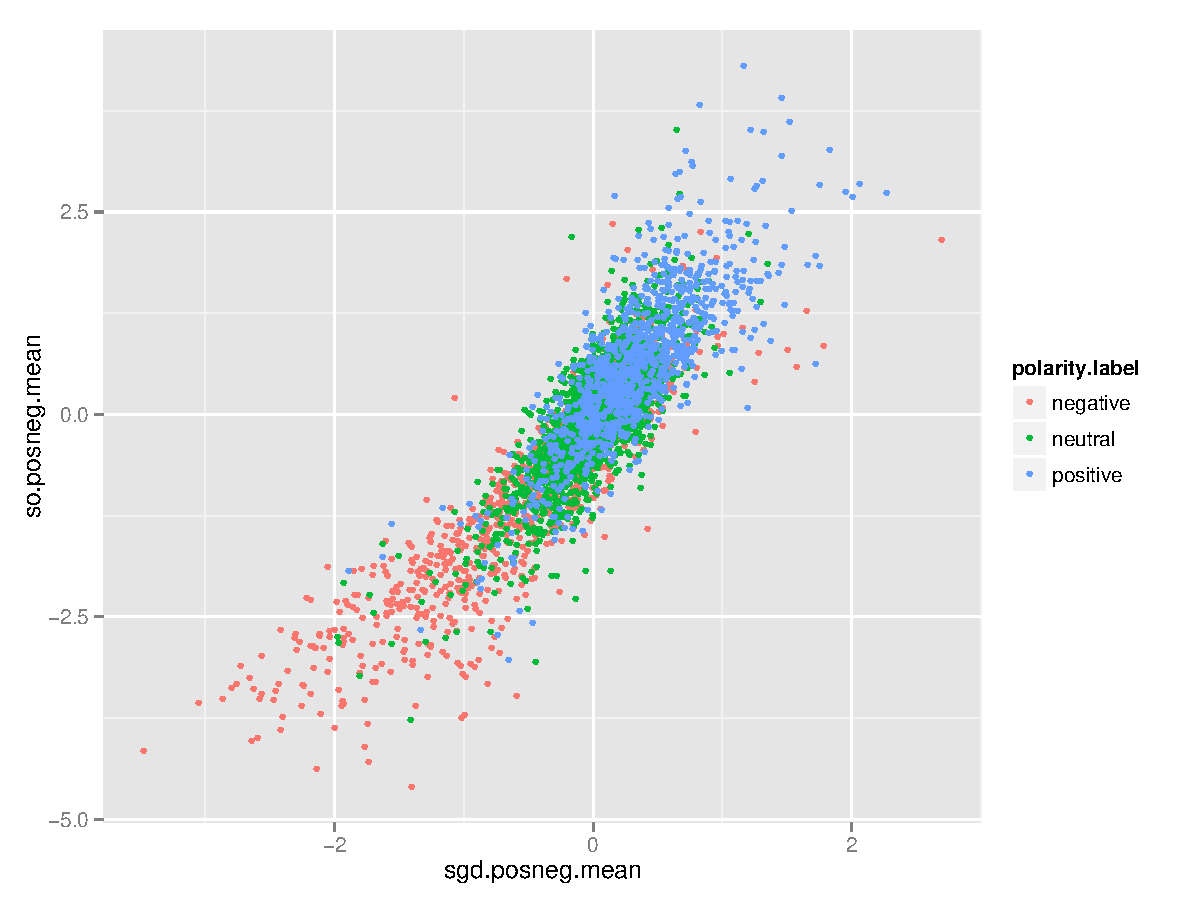
\includegraphics[width=7.5cm,height=6cm]{SGDSO.pdf}
	\caption{SO SGD}
	\label{fig:sosgd}
\end{figure}


From the figure we can observe that both variables are highly correlated with each other (0.858). We can also observe that as negative words tend to show low values of SGD and SO, positive words tend to show the opposite. Neutral words are more spread out and hard to distinguish. 


\begin{figure}[ht]
	\centering
	%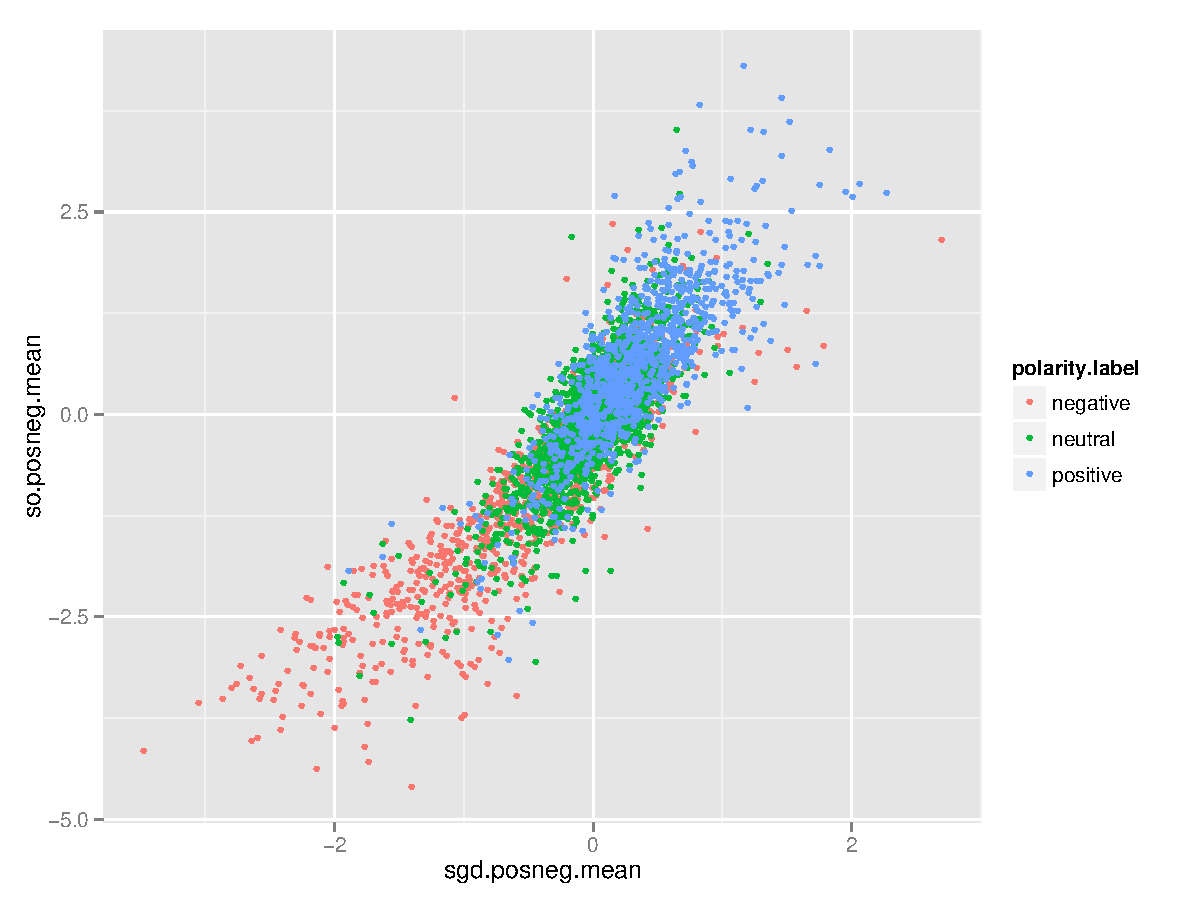
\includegraphics[scale=0.4]{SGDSO.pdf}
	 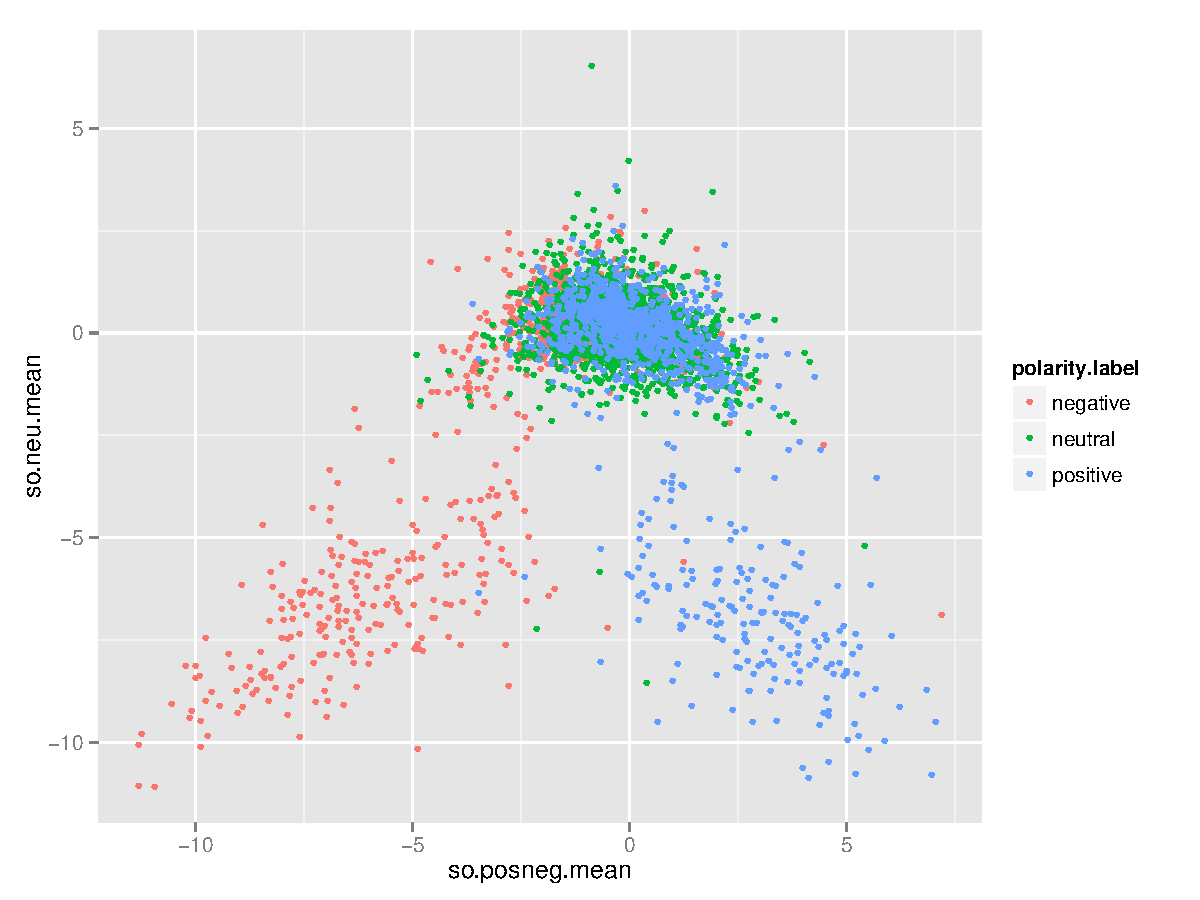
\includegraphics[width=7.5cm,height=6cm]{SOSO.pdf}
	\caption{SO SGD}
	\label{fig:soso}
\end{figure}





\begin{figure}[ht]
\begin{center}
\begin{tabular}{cc}
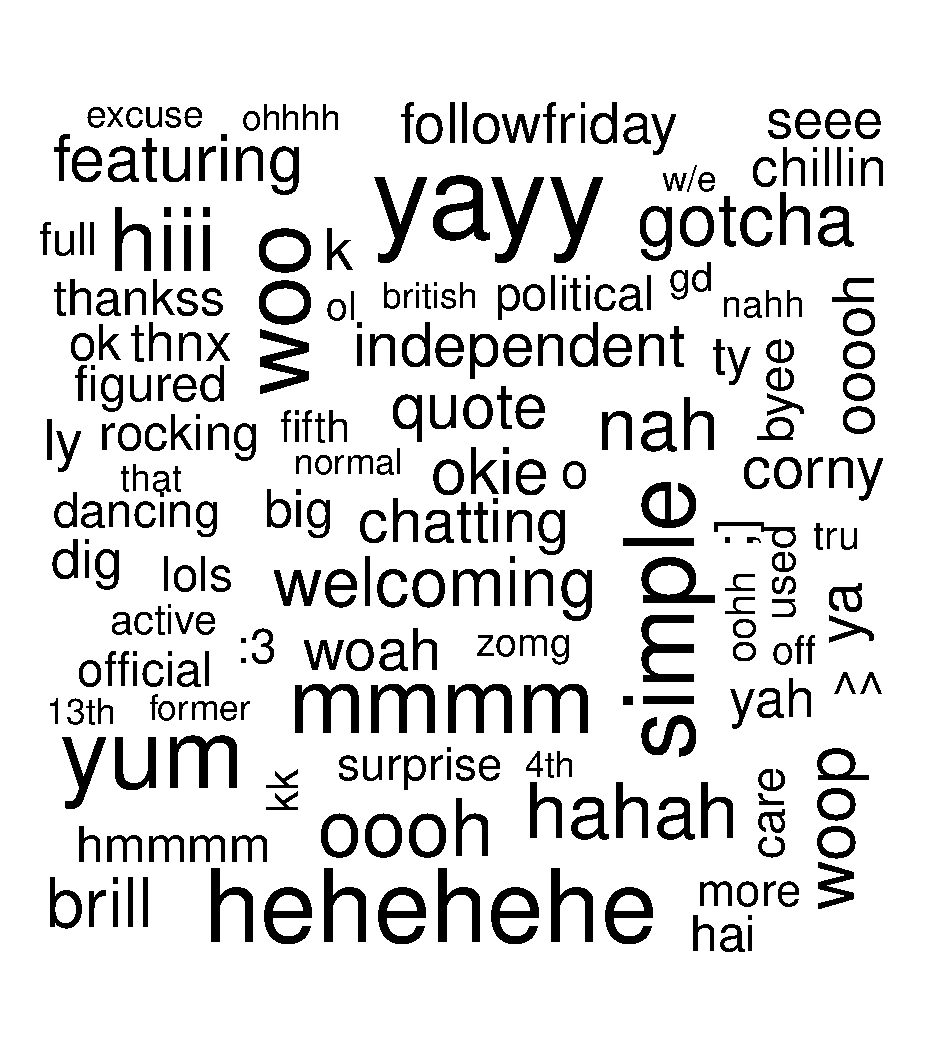
\includegraphics[scale=0.25]{poswords.pdf}
&
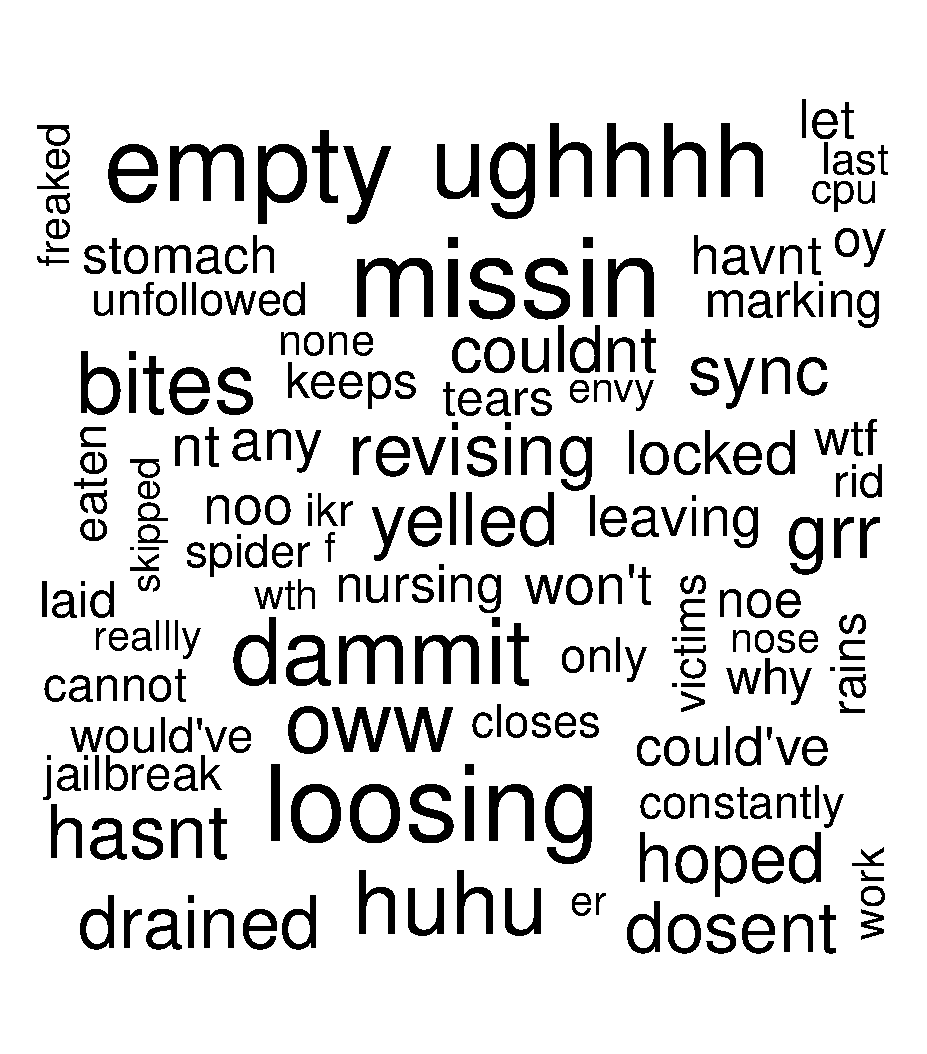
\includegraphics[scale=0.25]{negwords.pdf}\\
(a) & (b)  
\end{tabular}
\caption{\textbf{WordClouds of positive and negative words }}
\label{fig:scatter}
\end{center}
\end{figure}


% Discuss the intepretability problem produced by the consensus of methods



We study three word-level classification problems: 1) Neutrality: neutral vs non neutral words, 2) PosNeg: positive vs negative words, and 3) Polarity: neutral vs positive vs negative.

The information gain values obtained for the different attributes in relation to the three classification tasks are shown in Table~\ref{tab:infogains}.
 
 
\begin{table*}[htbp]
\begin{center}
\begin{tabular}{l|ccc|ccc|ccc}
\hline
Dataset & \multicolumn{3}{c|}{ED} & \multicolumn{3}{c|}{STS} & \multicolumn{3}{c}{CON} \\ \hline
 Task &  Neutrality & PosNeg & Polarity &  Neutrality & PosNeg & Polarity &  Neutrality & PosNeg & Polarity  \\ \hline
pos-tag &  0.062 & 0.017  & 0.071 & 0.068 & 0.016 & 0.076 & 0.049 & 0.014 & 0.056 \\ 
sgd.posneg.mean & \textbf{0.082}  & 0.233  &  0.200 & \textbf{0.104} & 0.276 & \textbf{0.246} & 0.070 & 0.247  & 0.207  \\ 
sgd.posneg.last & 0.057 & 0.177 & 0.155  & 0.086 & 0.258 & 0.221 &  0.073 & 0.248 & 0.205 \\ 
so.posneg.mean & 0.079 & \textbf{0.283} & \textbf{0.219}  & 0.081 & \textbf{0.301} & 0.232 & 0.088 & 0.305 & 0.256 \\ 
so.posneg.last & 0.069 & 0.279  &  0.211 & 0.084 & 0.300 & 0.240 & 0.094 & \textbf{0.323} & \textbf{0.264} \\ 
sgd.neu.mean & $\times$ & $\times$ & $\times$ & $\times$ & $\times$ & $\times$ & \textbf{0.103} & 0.009  & 0.106 \\ 
sgd.neu.last & $\times$ & $\times$  & $\times$ & $\times$ & $\times$ & $\times$ & \textbf{0.103} & 0.010 & 0.106 \\ 
so.neu.mean & $\times$ & $\times$  & $\times$ & $\times$ & $\times$ & $\times$ & \textbf{0.103} & 0.000 & 0.105 \\ 
so.neu.last & $\times$ & $\times$ & $\times$ & $\times$ & $\times$ & $\times$ & \textbf{0.103} & 0.000 & 0.105 \\ \hline
\end{tabular}
\end{center}
\caption{Information gain Values of main attributes}
\label{tab:infogains}
\end{table*}

 
 
 
 


We can observe that variables measuring the central tendency of the SO and SGD time series tend to be more informative than the ones measuring deviance. Moreover, the information gain values of these variables are much higher for PosNeg than for neutrality. As SGD and SO are competitive measures for neutrality, SO tends to be better for PosNeg. The average values of SO and SGD are better than the last values especially in SGD. We can also see that POS tags are useful for neutrality detection, but are useless for PosNeg. Therefore, we can conclude that positive and negative words have a similar distribution of POS tags. 


The accuracy of the classification experiments are presented in Table~\ref{tab:classres}. 








\begin{table*}[htbp]
\begin{center}
\begin{tabular}{l|l|l|l|l|l}
\hline \hline
\multicolumn{ 6}{c}{Accuracy } \\ \hline \hline
Dataset & SO & ALL & SGD.TS+POS & SO.TS+POS & SO+POS \\ \hline
ED-Neutrality & 61.52 $\pm$ 2.21 & \textbf{65.16 $\pm$ 2.09} $\circ$ & 64.55 $\pm$ 2.27 $\circ$ & 64.9 $\pm$ 2.14  $\circ$ & 64.18 $\pm$ 2.12 $\circ$ \\ 
ED-PosNeg & 74.78 $\pm$ 2.93 & \textbf{76.04 $\pm$ 2.72} & 73.61 $\pm$ 2.51 & 75.6 $\pm$ 2.84 & 74.99 $\pm$ 2.72 \\ 
ED-Polarity & 59.48 $\pm$ 2.29 & \textbf{61.93 $\pm$ 2.1 $\circ$} & 60.97 $\pm$ 1.96 & 61.73 $\pm$ 1.98 $\circ$ & 61.57 $\pm$ 2.04 $\circ$ \\  \hline
STS-Neutrality & 62.99 $\pm$ 2.03 & \textbf{66.2 $\pm$ 2.11 $\circ$} & 65.26 $\pm$ 2.34 $\circ$ & 65.73 $\pm$ 1.98 $\circ$ & 65.77 $\pm$ 2.09 $\circ$ \\ 
STS-PosNeg & \textbf{77.18 $\pm$ 2.88} & 76.98 $\pm$ 2.82 & 75.39 $\pm$ 2.89 $\bullet$ & 76.76 $\pm$ 2.89 & 76.98 $\pm$ 2.71 \\ 
STS-Polarity & 60.2 $\pm$ 2.23 & \textbf{62.74 $\pm$ 1.52} $\circ$ & 62.34 $\pm$ 1.61 $\circ$ & 62.14 $\pm$ 1.73 $\circ$ & 62.1 $\pm$ 1.78 $\circ$ \\  \hline
CON-Neutrality & 61.07 $\pm$ 2.72 & \textbf{66.26 $\pm$ 2.54} $\circ$ & 64.18 $\pm$ 2.24  $\circ$ & 65.96 $\pm$ 2.48 $\circ$ & 64.80 $\pm$ 2.46 $\circ$ \\ 
CON-PosNeg & 75.82 $\pm$ 2.97 & \textbf{76.50 $\pm$ 3.1} & 70.20 $\pm$ 2.92 $\bullet$  & 76.06 $\pm$ 3.11  & 75.59 $\pm$ 2.95 \\ 
CON-Polarity & 58.42 $\pm$ 1.99 & 61.21 $\pm$ 2.13 $\circ$ & 58.84 $\pm$ 2.02 & \textbf{62.01 $\pm$ 2.46} $\circ$ & 60.32 $\pm$ 2.44 $\circ$ \\ \hline \hline
\multicolumn{ 6}{c}{Weighted area under ROC } \\ \hline \hline
Dataset & SO & ALL & SGD.TS+POS & SO.TS+POS & SO+POS \\ \hline
ED-Neutrality & 0.62 $\pm$ 0.02 &  \textbf{0.65 $\pm$ 0.02} $\circ$ & \textbf{0.65 $\pm$ 0.02} $\circ$  & \textbf{0.65 $\pm$ 0.02} $\circ$ & 0.64 $\pm$ 0.02 $\circ$ \\ 
ED-PosNeg & 0.74 $\pm$ 0.03 & \textbf{0.75 $\pm$ 0.03} & 0.71 $\pm$ 0.03 $\bullet$ & 0.74 $\pm$ 0.03 & 0.73 $\pm$ 0.03 \\ 
ED-Polarity & 0.62 $\pm$ 0.02 &  \textbf{0.65 $\pm$0.02} $\circ$ & 0.64 $\pm$ 0.02 & \textbf{0.65 $\pm$ 0.02} $\circ$ & 0.64 $\pm$ 0.02 $\circ$ \\ \hline
STS-Neutrality & 0.63 $\pm$ 0.02 & \textbf{0.67 $\pm$ 0.02} $\circ$             & 0.66 $\pm$ 0.02 $\circ$  & 0.66 $\pm$ 0.02 $\circ$ & 0.66 $\pm$ 0.02$\circ$ \\ 
STS-PosNeg & \textbf{0.77 $\pm$ 0.03} &  \textbf{0.77 $\pm$ 0.03} & 0.75 $\pm$ 0.03 $\bullet$ & \textbf{0.77 $\pm$ 0.03} & \textbf{0.77 $\pm$ 0.03} \\ 
STS-Polarity & 0.64 $\pm$ 0.02 & \textbf{0.66 $\pm$ 0.01} $\circ$  & 0.65 $\pm$ 0.02 $\bullet$  & \textbf{0.66 $\pm$ 0.02} $\circ$ & \textbf{0.66 $\pm$ 0.02} $\circ$ \\ \hline
CON-Neutrality & 0.61 $\pm$ 0.03 & \textbf{0.67 $\pm$ 0.03}  $\circ$ & 0.65 $\pm$ 0.02 $\circ$ & 0.66 $\pm$ 0.02  $\circ$ & 0.65 $\pm$ 0.02 $\circ$ \\ 
CON-PosNeg & \textbf{0.76 $\pm$ 0.03} & \textbf{0.76 $\pm$ 0.03} & 0.70 $\pm$ 0.03 $\bullet$ & \textbf{0.76 $\pm$ 0.03} & 0.75 $\pm$ 0.03 \\ 
CON-Polarity & 0.63 $\pm$ 0.02 & 0.65 $\pm$ 0.02 $\circ$ & 0.62 $\pm$ 0.02  & \textbf{0.66 $\pm$ 0.02}  $\circ$ & 0.64 $\pm$ 0.02 $\circ$ \\ \hline
\end{tabular}
\caption{World level classification accuracies} 
\end{center}
\label{}
\end{table*}







All the experiments were done using RBF SVM with a grid search procedure for parameter tuning. The evaluation was done using 10 times 10-folds-cross-validation and different sub-sets of attributes were compared.  All the methods are compared with the baseline of using the last value of the semantic orientation through a paired t-student test with an alpha level of $0.1$.   
Results indicate that the combination of all the features leads a significant improvement in accuracy for neutrality classification.  In the PosNeg classification task we can see that the baseline is very strong. This suggests that the SO is very good for discriminating between positive and negative words. However, we can observe that when all attributes are combined a statistically significant improvement is achieved.





\begin{table*}[htbp]

\begin{center}
\begin{tabular}{l|l|l|l|l|l}
\hline \hline
\multicolumn{ 6}{c}{Accuracy } \\ \hline \hline
Dataset & Baseline & ED & S140 & Cons & Combination \\ \hline
6-coded & 71.79 $\pm$ 2.79 & 74.91 $\pm$ 2.56 $\circ$ & 75.11 $\pm$ 2.66 $\circ$ & 73.4 $\pm$ 2.81 $\circ$ & \textbf{75.74 $\pm$ 2.46} $\circ$ \\ 
Sanders & 71.43 $\pm$ 3.76 & 77.17 $\pm$ 3.68 $\circ$ & 77.32 $\pm$ 4.09 $\circ$ & 77.58 $\pm$ 3.52 $\circ$ & \textbf{77.74 $\pm$ 3.57} $\circ$ \\ 
SemEval & 76.81 $\pm$ 1.22 & 76.66 $\pm$ 1.38 & 77.7 $\pm$ 1.25 $\circ$ & 77.66 $\pm$ 1.34 $\circ$ & \textbf{78.37 $\pm$ 1.37} $\circ$ \\ \hline \hline
\multicolumn{ 6}{c}{Weighted area under ROC } \\ \hline \hline
Dataset & Baseline & ED & S140 & Cons & Combination \\ \hline
6-coded & 0.77 $\pm$ 0.03 & 0.82 $\pm$ 0.03 $\circ$ & 0.82 $\pm$ 0.02 $\circ$ & 0.81 $\pm$ 0.03 $\circ$ & \textbf{0.83 $\pm$ 0.02} $\circ$ \\ 
Sanders & 0.77 $\pm$ 0.04 & 0.83 $\pm$ 0.04 $\circ$ & 0.84 $\pm$ 0.04 $\circ$ & 0.83 $\pm$ 0.04 $\circ$ & \textbf{0.85 $\pm$ 0.04} $\circ$ \\ 
SemEval & 0.77 $\pm$ 0.02 & 0.81 $\pm$ 0.02 $\circ$ & 0.83 $\pm$ 0.02 $\circ$ & 0.8 $\pm$ 0.02 $\circ$ & \textbf{0.83 $\pm$ 0.02} $\circ$ \\ \hline
\end{tabular}
\caption{Message Level Polarity Classification Accuracies using word probabilities}
\end{center}
\label{}
\end{table*}





\begin{table*}[htbp]
\begin{center}
\begin{tabular}{l|l|l|l|l|l}
\hline
\hline
\multicolumn{ 6}{c}{Accuracy } \\ \hline \hline
Dataset & Baseline & ED & S140 & Cons & Combination \\ \hline
6Coded & 71.79 $\pm$ 2.79 & 76.57 $\pm$ 2.3 $\circ$ & 75.28 $\pm$ 2.5 $\circ$ & 74.74 $\pm$ 2.51 $\circ$ & \textbf{77.36 $\pm$ 2.53} $\circ$ \\ 
Sanders & 71.43 $\pm$ 3.76 & \textbf{76.78 $\pm$ 3.99} $\circ$ & 75.83 $\pm$ 4.19 $\circ$ & 75.81 $\pm$ 4.17 $\circ$ & 76.07 $\pm$ 3.92 $\circ$ \\ 
SemEval & 76.81 $\pm$ 1.22 & 78.23 $\pm$ 1.3 $\circ$ & 77.07 $\pm$ 1.18 & 78.18 $\pm$ 1.25 $\circ$ & \textbf{79.4 $\pm$ 1.29} $\circ$ \\ \hline \hline
\multicolumn{ 6}{c}{Weighted area under ROC } \\ \hline \hline
Dataset & Baseline & ED & S140 & Cons & Combination \\ \hline 
6Coded & 0.77 $\pm$ 0.03 & 0.84 $\pm$ 0.02 $\circ$ & 0.82 $\pm$ 0.03 $\circ$ & 0.81 $\pm$ 0.03 $\circ$ & \textbf{0.85 $\pm$ 0.02} $\circ$ \\ 
Sanders & 0.77 $\pm$ 0.04 & 0.83 $\pm$ 0.04 $\circ$ & 0.82 $\pm$ 0.04 $\circ$ & 0.82 $\pm$ 0.04 $\circ$ & \textbf{0.84 $\pm$ 0.04} $\circ$ \\ 
SemEval & 0.77 $\pm$ 0.02 & 0.83 $\pm$ 0.02 $\circ$ & 0.82 $\pm$ 0.02 $\circ$ & 0.82 $\pm$ 0.02 $\circ$ & \textbf{0.85 $\pm$ 0.02} $\circ$ \\ \hline
\end{tabular}
\end{center}
\caption{Message Level Polarity Classification Accuracies using word probabilities no Outliers}
\label{}
\end{table*}





\section{Conclusions}\label{sec:conc}


\bibliographystyle{abbrv}
\bibliography{bio}


\end{document}
